\part{Empirical}
\chapter{Context}
In the center of Africa we find the country known as Rwanda. A very small country, only \(26338 km^2\). This would be about 7\% of Norway. 
Their population is estimated to be around 12 million wich makes it about 420 people pr. square kilometer. 
Rwanda is made up of 5 provinces, east, west, north, south and Kigali. 
Each province is again divided into districts and there is a total of 30 districts. Under districts there is a total of 416 sectors\cite{1}.
\begin{figure}
\centering
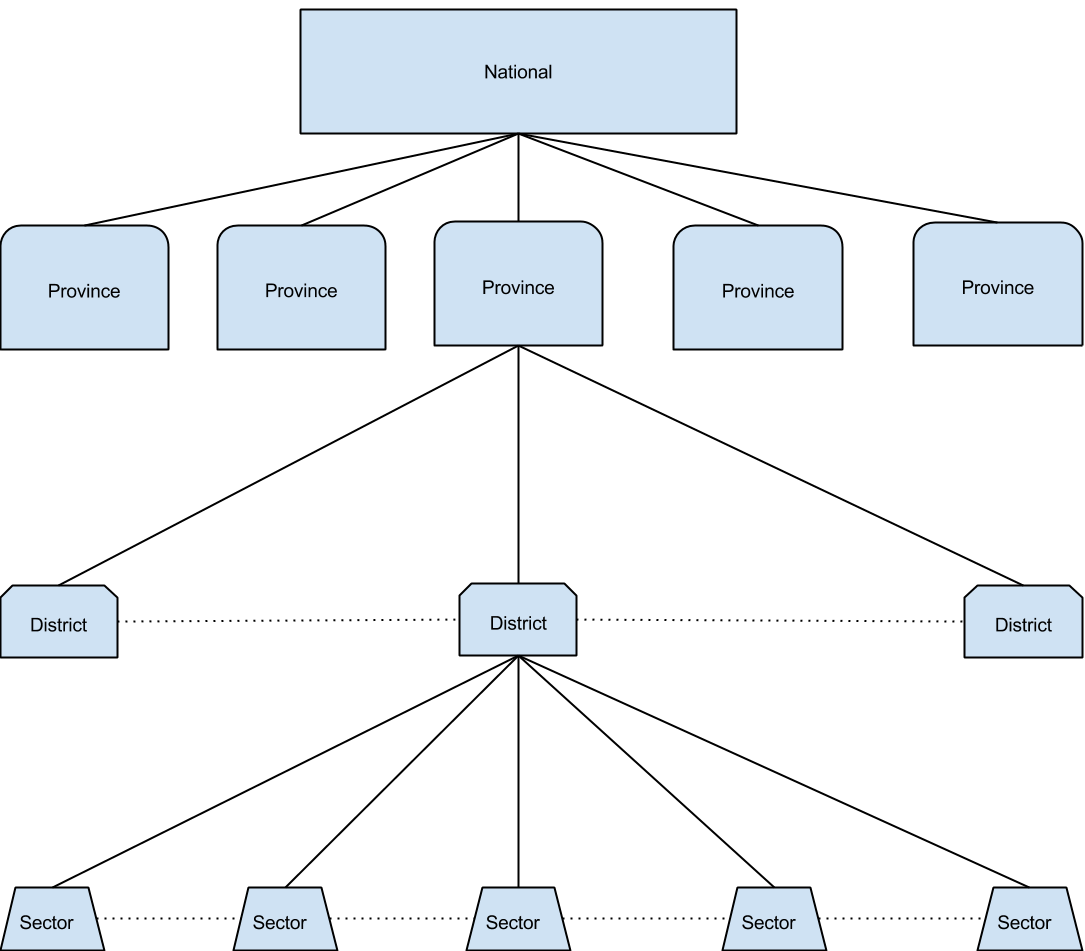
\includegraphics[width=12cm]{empirical/images/rwanda_administrative_division}
\caption{Rwanda Administrative Division}
\end{figure}
It lies in the center of Africa with Uganda at the north, Tanzania to the east, Burundi at the south and the Democratic Republic of Congo in the west. Because of its location it works perfect as a gateway to all countries in Africa. 
And because of the stable environment comparing to the neighboring contries it is even more attractive for foreigners doing business in Africa making it the `Singapore of Africa'.

Rwanda has a goal of transforming to a knowledge based economy with Information and Communication Technology as their field of knowledge. This means basicly that they want to offer ICT services for other kind of resources. 
They want to be the regional center for the training of top quality ICT\nomenclature{ICT}{Information and Communication Technology} professionals.
This will hopefully in turn create wealth, jobs and entreprenaurs. From their perspective they have some competetive advantages in order to achieve this wich include:
\begin{itemize}
\item Cheap labor compared to other countries in the Region
\item Young and dynamic workforce (98\% of the population is under 50 years and 43\% is under 16 years)
\item Most favorable business environment in the Region (8th best place to do business in the world 2012)
\item Low levels of corruption - Zero tolerance (Transparency international Bribery index 2012 ranked Rwanda as least bribery prone in the EAC)
\item World class ICT infrastructure
\item Strong \& visionary leadership
\item Bi-lingual business environment (French and English)
\end{itemize}
\cite{2}

\section{Information Technology focus in Rwanda}

\begin{figure}
\centering
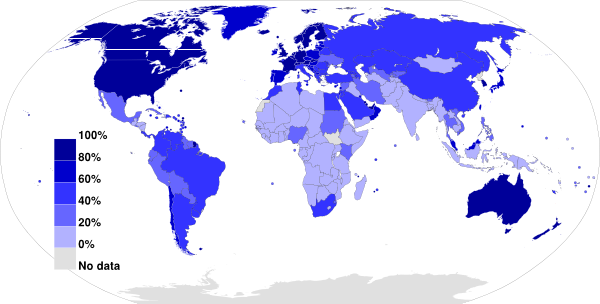
\includegraphics[width=12cm]{empirical/images/internet_penetration_2012}
\caption{Global Internet Penetration in 2012 \cite{3}}
\label{fig:global_internet_penetration_2012}
\end{figure}
\begin{figure}
\centering
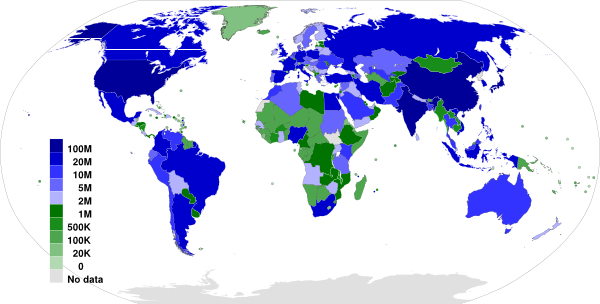
\includegraphics[width=12cm]{empirical/images/internet_users_2012}
\caption{Global Internet Users in 2012 \cite{3}}
\label{fig:global_internet_users_2012}
\end{figure}
Rwanda has an internet penetration of 7\% in 2012. In Africa there is internet penetration is 15.6\% and for the world it is 34.3\% (See ~\ref{fig:global_internet_penetration_2012}).
The neighbouring countries, Uganda has 2.6\%, Tanzania 12.0\%, Burundi 1.7\% and the Democratic Republic of Congo with 1.2\%\cite{4}. Rwanda grew from 1\% to 7\% from 2000 to the end of 2011\cite{2}.
More interesting is the mobile broadband development in Rwanda. The subscriber base accounts for 48.1\% of the population and the network coverage accounts for 99.79\% of the country.
The government of Rwanda has made the decision to become an ICT hub in Africa. Therefore alot of resources and attention is focused on developing knowledge in the field of ICT. 
They are in 2012 ranked among the top 6 developing countries when it comes to dynamic performance in ICT development\cite{5}.
\subsection{The ICT park project}
As of january 2013 the Rwandian government is planning to set up an ICT park through the Rwanda Development Board.
This park will host technological training, industries research and development. The ICT park will support the growth of the following clusters:
\begin{itemize}
\item Energy
\item Internet, multimedia and mobile telecommunication
\item Knowledge
\item E-Government
\item Financial
\item ICT Service and export
\end{itemize}
\cite{2}

\section{Health Information Systems in Rwanda}
The government instance that has the responsibility to maintain and manage health information data is the Ministy of Health. Here there is a team that maintains the Health Management Information System.
The HMIS \nomenclature{HMIS}{Health Management Information System} is built on open source District Health Informaiton System 2. 
The health ministry has made some modifications so that there is in fact 4 instances of DHIS2\nomenclature{DHIS2}{District Health Information System 2} running for different purposes.
\begin{figure}
\centering
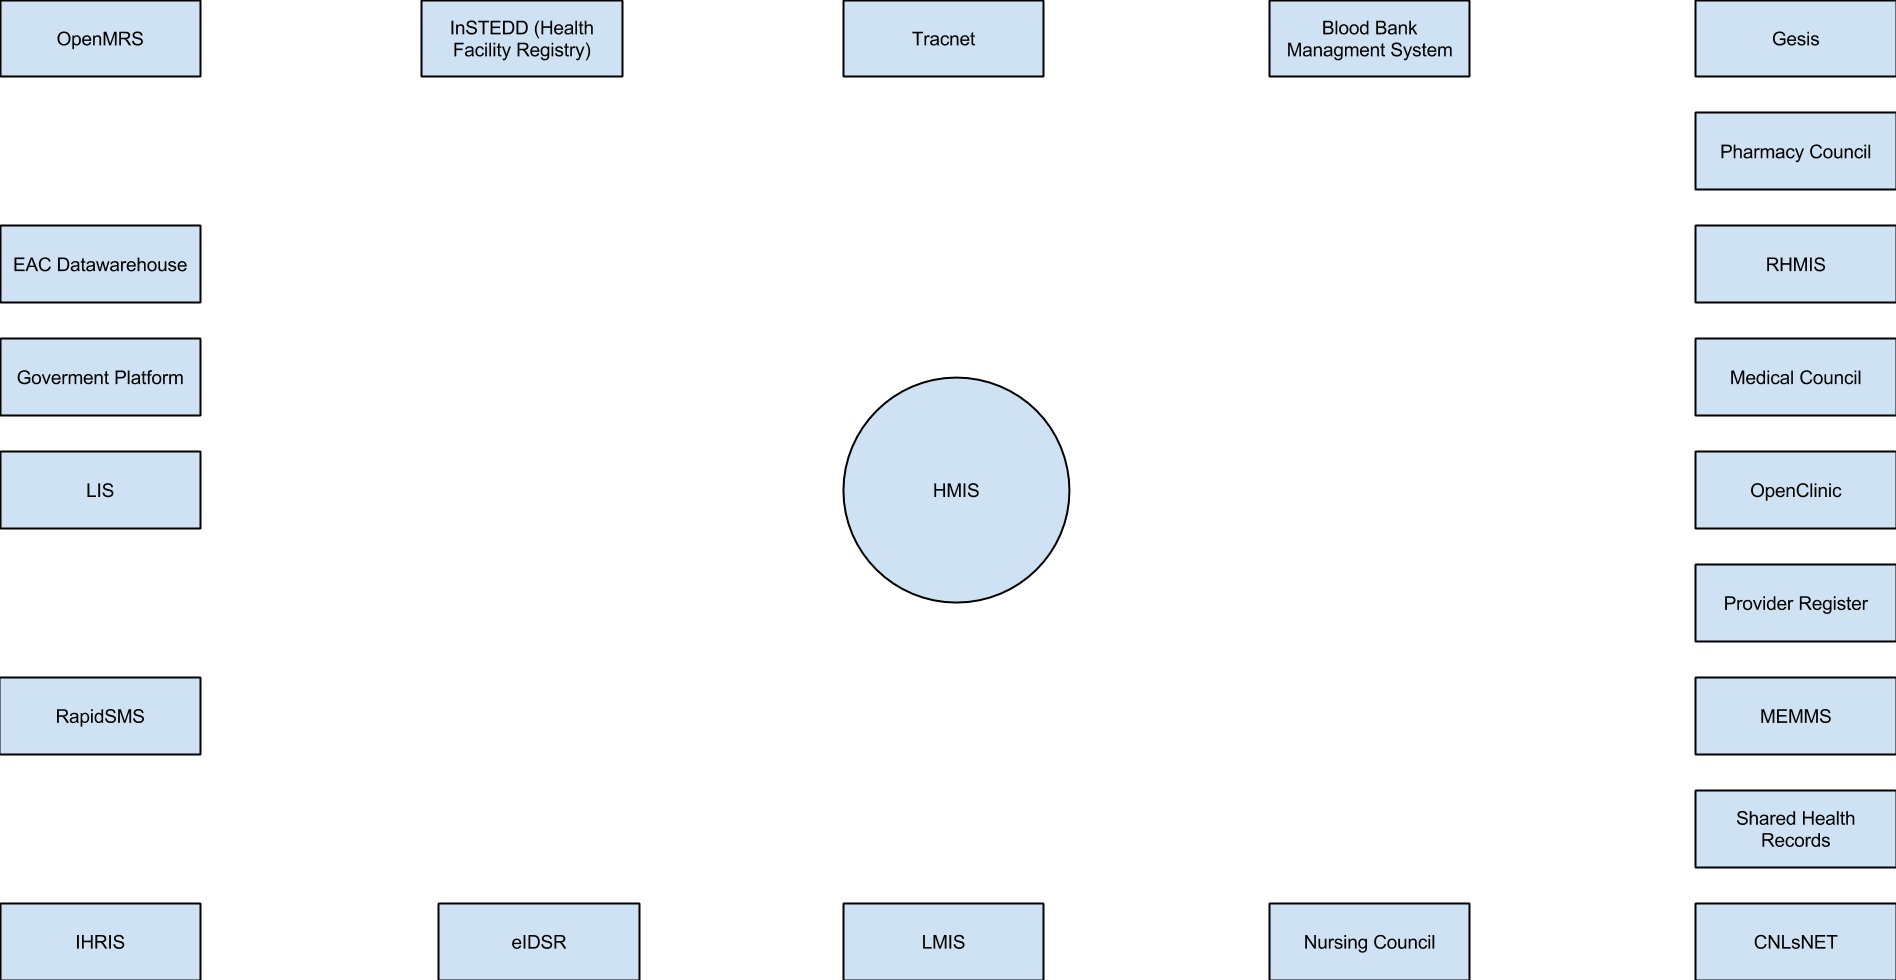
\includegraphics[width=12cm]{empirical/images/context.png}
\caption{Systems Currently in Use 2013}
\label{fig:systems_currently_in_use_2013}
\end{figure}
Besides the HMIS there are alot of systems that runs and has critical tasks that is not yet supported solely by DHIS2, see ~\ref{fig:systems_currently_in_use_2013}. These systems has varying tasks, but are all in some way related to HMIS.
Sharing data between these systems is crucial for maintaining an overview of the health status in all of Rwanda. 


\chapter{Method}

\chapter{Case}
\section{Health Information System Programme}
\subsection{About}

\subsection{History}

\section{District Health Information System}
\subsection{About}

\subsection{Modules}
\subsection{Usage}
\subsubsection{Use Case}

\section{Inforamation Systems in Rwanda}
\subsection{Current situation}

\subsection{Health Ministy Information System}
\subsection{DHIX}
\subsubsection{Apache Camel}
\subsection{Malaria Surveliance}
\subsubsection{Sentinel Surveliance}
\subsubsection{Active Surveliance}
\subsection{Voxivia}

